\documentclass[a4paper,12pt,one side,titlepage]{report}


%en francais
\usepackage[T1]{fontenc}
\usepackage{lmodern}
\usepackage[utf8]{inputenc}
\usepackage[francais]{babel}



\usepackage{listings}
\usepackage{geometry}
\usepackage{graphicx}
\usepackage{eurosym}
\usepackage{url}
\usepackage{pdfpages}
\usepackage[acronym]{glossaries}
\usepackage{hyperref}
\usepackage{graphicx}
%\usepackage[top=2.5cm,bottom=2.5cm,left=2.5cm,right=2.5cm]{geometry}
%\hypersetup{pdfborder=0}




\newglossaryentry{firewall}
{
	name={firewall},
	description={Protection pour serveur}
}

\newglossaryentry{naxsi}
{
	name={naxsi},
	description={Un type de firewall}
}



\makeglossaries
\begin{document}
%\includepdf[pages = {1-1}]{./pdf/1stpage.pdf}
%\includepdf[pages = {1-1}]{./pdf/pagegarde.pdf}


\begin{titlepage}
\begin{center}

\textsc{\LARGE Licence ASRALL}\\[1.5cm]

\textsc{\Large Exposé technique}\\[5.9cm]

% Title
{ \huge \bfseries Fully Automatic Installation\\[1.9cm] }

% Author and supervisor
\noindent
\begin{minipage}{0.4\textwidth}
\begin{flushleft} \large
François \textsc{Dupont}
\end{flushleft}
\end{minipage}%
\begin{minipage}{0.4\textwidth}
\begin{flushright} \large
Florent \textsc{Fillion}
\end{flushright}
\end{minipage}

\vfill

% Bottom of the page
{\large \today}

\end{center}
\end{titlepage}


%Page table des matières
\tableofcontents

%Introduction
\chapter{Introduction}
\section{Objectifs}
\subsection{Définition}
\textit{Fully Automatic Installation} ou \textsc{FAI} est un logiciel libre, inspiré de son équivalent \textsc{Solaris}, \textsc{Jumpstart}. Il permet d'installer et de configurer un système d'exploitation Linux sur une ou plusieurs machines, en utilisant un infrastructure client serveur, de façon rapide et automatisé.

Il est à noter que \textsc{FAI} n'est pas interactif contrairement à d'autres logiciels remplissant sensiblement la même fonction. Ce logiciel est également considéré comme mature (il en est à sa 4\textsuperscript{ème} itération majeure (4.0) et est développé de façon continue depuis 1999.

\subsection{Utilité}
\textsc{FAI} s'adresse particulièrement aux administrateurs ayant à gérer un grand parc de machine sous Linux, que ce parc soit \textit{virtualisé} ou physique (et même des \textit{chroot}s).

\section{Histoire}


\section{Concepts}
Cette partie pourrait avoir sa place dans le chapitre traitant de la technique à proprement parler, cependant, il nous semble essentiel d'exposer les principes fondamentaux (et simples une fois assimilés) de \textsc{FAI}.



\chapter{Technique}

\chapter{Alternatives}
Il existe plusieurs alternatives à FAI, tels que Jumpstart(Solaris), Kickstart(RedHat), Rembo, ou encore ...................

\section{Jumpstart}
Jumpstart a été créé par Sun Microsystems, qui fut ensuite racheté en 2009 par Oracle Corporation. C'est un outil permettant d'automatiser l'installation d'une ou plusieurs machines utilisant Solaris comme système d'exploitation.\\
La configuration de Jumpstart s'effectue à l'aide de plusieurs fichiers :\\
\begin{itemize}
  \item Le fichier \textit{profile} qui définit les partitions de disques.
  \item Les fichiers \textit{rules} et \textit{rules.ok} qui définissent les règles correspondant à un profil particulier de client à installer.
  \item Des scripts s'exécutant avant et après l'installation de la machine cliente.
  \item Le fichier \textit{sysidcfg} qui définit les informations de configuration du client, comme par exemple son nom d'hôte, son adresse IP, etc...
  \item Le fichier \textit{/etc/bootparams} qui est utilisées par les machines clientes pour démarrer.
  \item Le fichier \textit{/etc/ethers} qui contient les mappages d'adresses MAC pour les clients.\\
\end{itemize}
Lors de l'installation, le programme Jumpstart va tenter de faire correspondre le sytème à installer aux règles définies dans le fichier \textit{rules.ok}. Il lit donc ces règles, de la première à la dernière. Lorsque qu'une correspondance est établie entre un système et une règle, le programme JumpStart interrompt la lecture du fichier \textit{rules.ok} et commence l'installation du système d'après le profil correspondant à la règle associée.\\
\begin{center}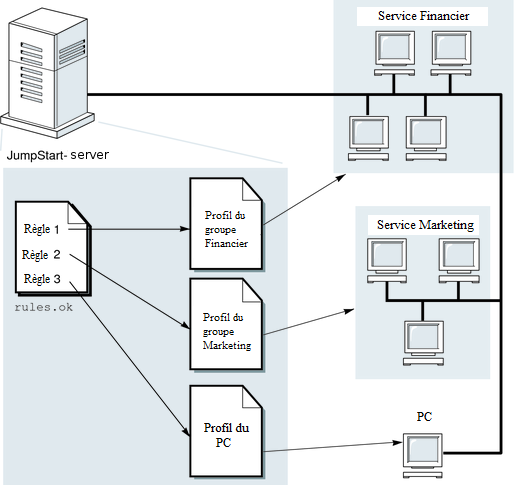
\includegraphics[scale=0.7]{./img/jumpstart2.png}\end{center}

Un serveur DHCP peut également être mis en place sur le serveur Jumpstart afin d'attribuer automatiquement une configuration IP aux machines clientes.\\

Voici un schéma représentant brièvement les requêtes effectuées entre les clients et le serveur lors du démarrage de l'installation :\\
\begin{center}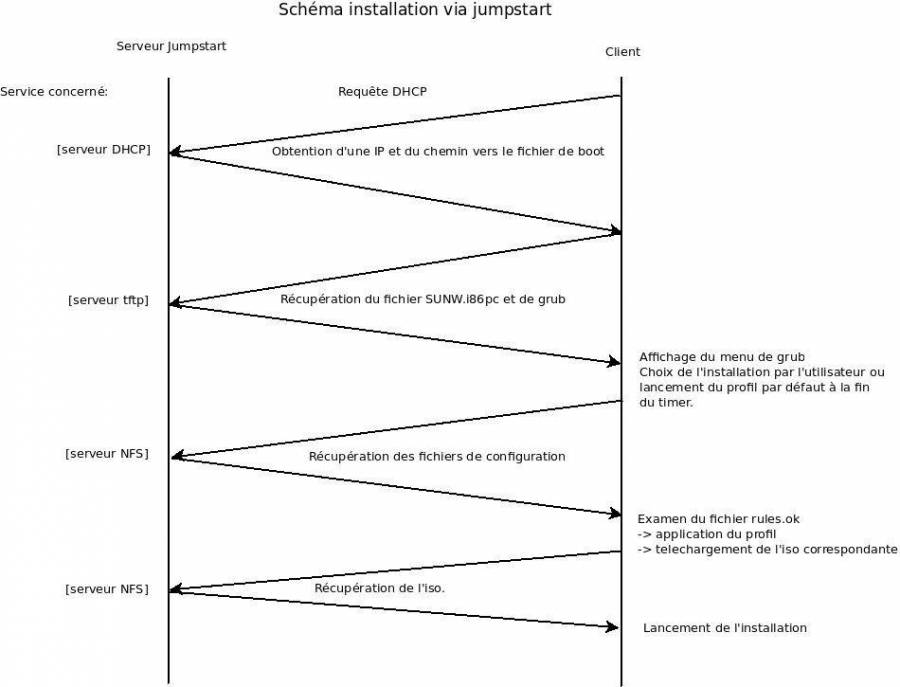
\includegraphics[scale=0.4]{./img/jumpstart.jpeg}\end{center}
\subsubsection{Configuration du Serveur Jumpstart}
Voici la liste des tâches à effectuer lors de la préparation à une installation JumpStart :\\
\begin{itemize}
  \item Créer un répertoire JumpStart\\
  \item Ajouter des règles pour chaque groupe dans le fichier \textit{rules} :\\
Chaque règle définit un groupe d'après un ou plusieurs attributs système. La règle lie chaque groupe à un profil.\\
  \item Créer un profil pour chaque règle :\\
Un profil est un fichier texte qui définit l'installation du logiciel Solaris, et indique par exemple le groupe de logiciels devant être installé sur un système. À chaque règle correspond un profil qui définit la procédure d'installation du logiciel Solaris sur un système. Ce profil est utilisé dès qu'une correspondance est établie entre une règle et un système déterminés.\\Généralement, on définit un profil pour chaque règle. Le même profil peut toutefois être utilisé dans plusieurs règles.\\
  \item Valider le fichier \textit{rules} :\\
Le fichier \textit{rules.ok} est une version générée du fichier \textit{rules} qu'utilise JumpStart pour détecter le système à installer avec un profil. Le fichier \textit{rules} se valide par l'intermédiaire d'un script \textit{check}.
\end{itemize}

\section{Kickstart}
Kickstart a été créé par RedHat afin d'automatiser l'installation de Fedora et Red Hate Enterprise Linux. Sa configuration s'effectue dans un fichier texte unique contenant une liste d'éléments, chacun identifié par un mot-clé. Ces éléments correspondent aux réponses à toutes les questions qui devraient normalement être posées lors d'une installation typique.\\
Ce fichier peut être créé manuellement en partant d'un fichier vierge puis en écrivant les directives une par une.
Cependant, et contrairement à FAI, il existe une interface utilisateur graphique, "Kickstart Configuration", permettant ainsi une configuration plus simple puisque il n'est pas nécessaire de se rappeler de la syntaxe exacte des fichiers :\\
\begin{center}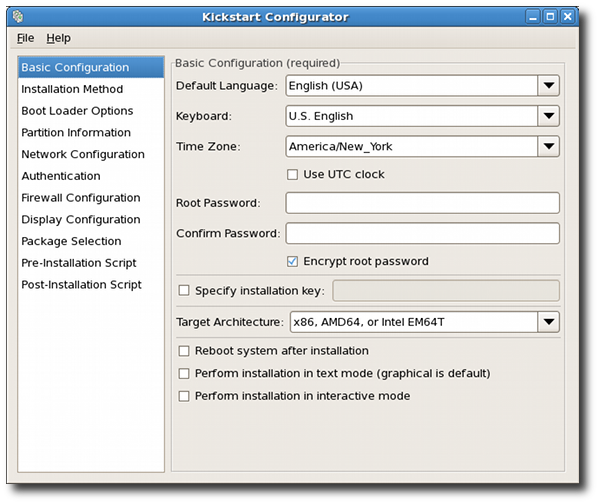
\includegraphics[scale=0.5]{./img/kickstart.png}\end{center}
.......................

\section{Rembo}
Rembo est le successeur de BPBatch. Il a été créé par "Rembo Technology", une société suisse spécialisée dans les outils de gestion applicative et de virtualisation de serveurs, qui fut ensuite rachetée en 2006 par IBM. Rembo est un environnement de déploiement d'applications qui permet d'installer rapidemment et en même temps, n machines du même type. Il peut s’exécuter sur Windows, Linux ou encore FreeBSD et s’appuie sur un serveur DHCP. Les machines clientes doivent donc supporter PXE et auront dont exactement la même installation. L'installation s'appuie sur l'utilisation d'une platine virtuelle, sur laquelle on sélectionne les programmes à installer. La procédure est ensuite entièrement automatique, et personnalisable à l'infini. Une machine virtuelle est créée à chaque installation puis est effacée lorsque le processus est terminé.

\chapter{Sources}
\begin{itemize}
  \item http://fai-project.org/\\\\
  \item https://docs.oracle.com/
\end{itemize}

\end{document}
